%!TEX root = ../RASD/main.tex
\newpage
\subsection{Alloy} % (fold)
In this section we provide an Alloy model for the \emph{system-to-be}.\\
The Alloy model includes all major requirements and constrains and checks the consistency of the most important components of the application.


\lstinputlisting[language=alloy]{../alloy/alloymodel.als}
\newpage

\subsubsection{Model considerations} % (fold)
\label{ssub:model_considerations}

\begin{landscape}
\begin{figure}[h!t]
\caption{Alloy model}
	\noindent\makebox[\textwidth]{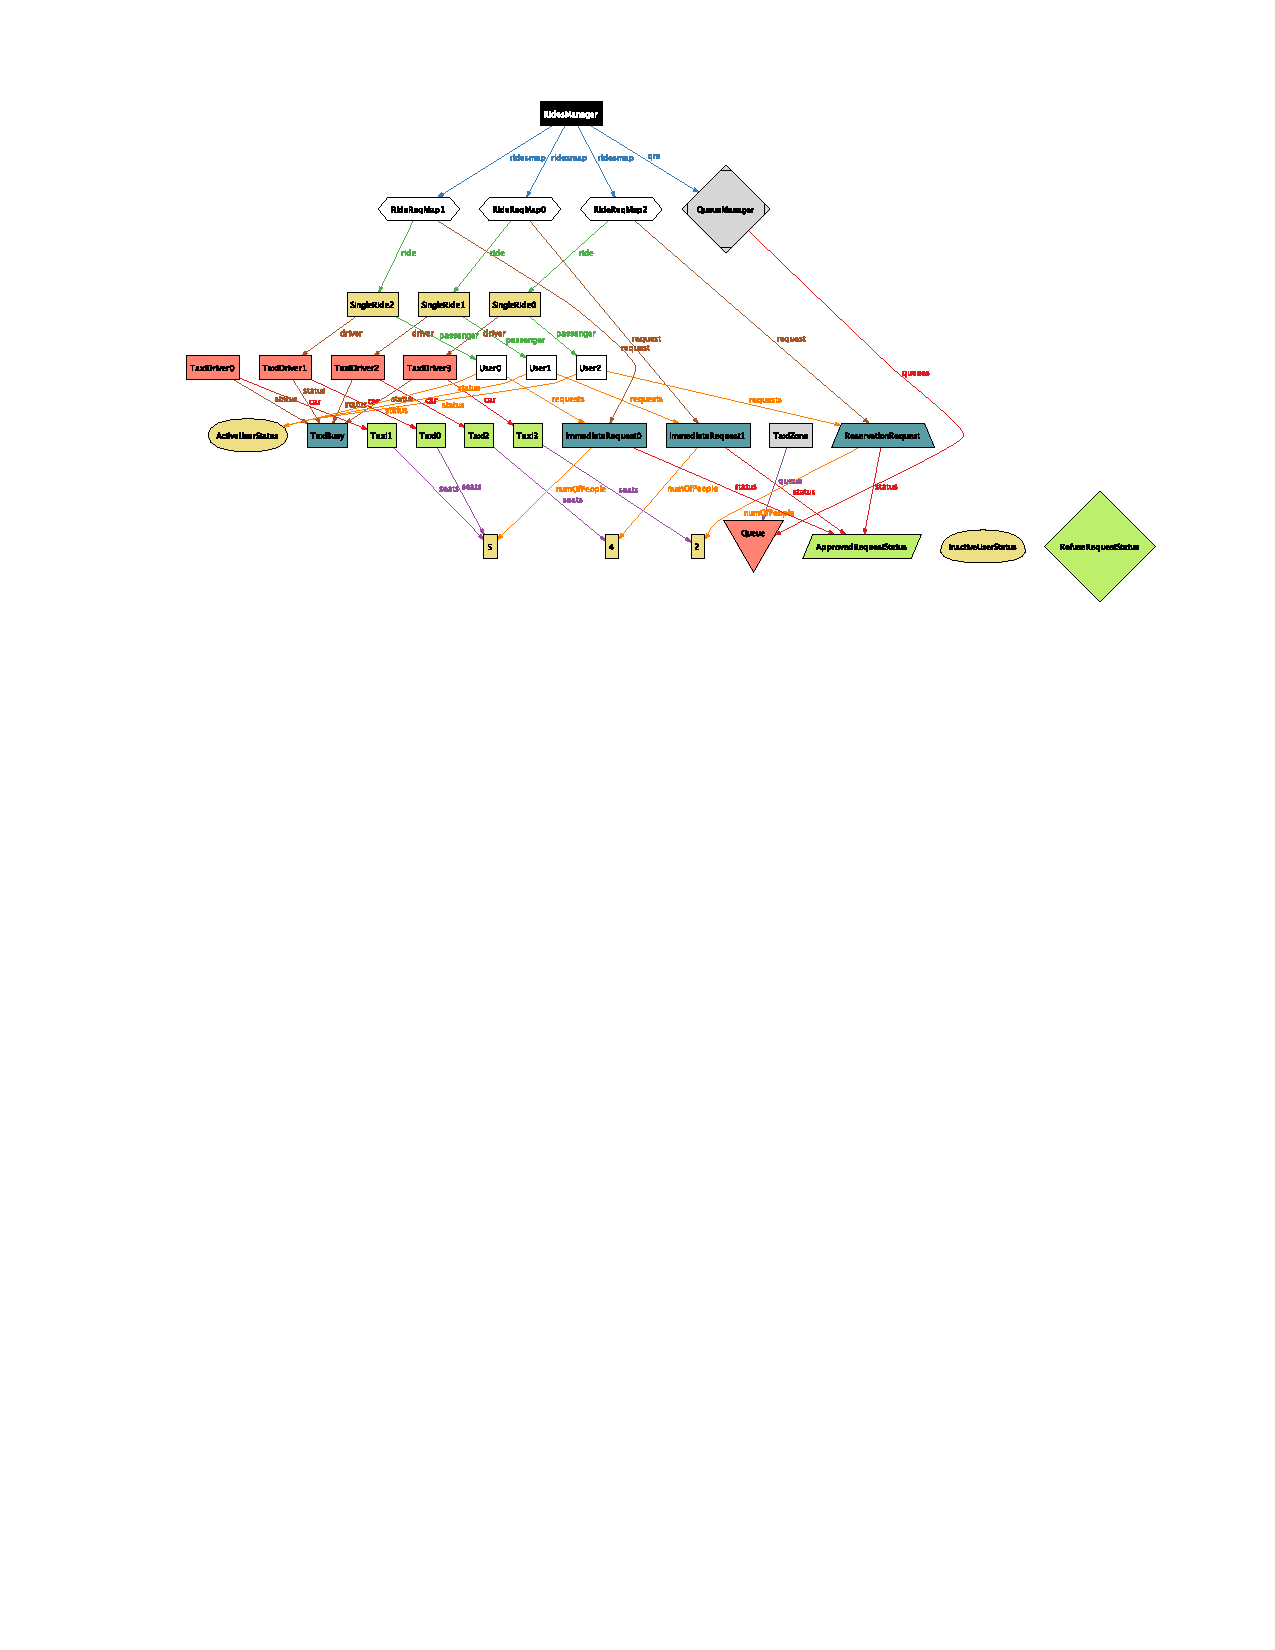
\includegraphics[width=\paperwidth]{alloy/alloyworld}}
\centering
\end{figure}
\end{landscape}

% subsubsection model_considerations (end)

